%% Paper title.
\title[Decision-Support for Urban Search \& Rescue Planning]{Decision-Support for Urban Search \& Rescue Mission Planning through Visualization-Based Analysis}

\author[\#255]{Submission ID \#255}
%\author[A. Bock et al.] {
%    Alexander Bock$^1$, Jonas Lundberg$^2$, Alexander Kleiner$^3$, and Timo Ropinski$^1$ \\
%    $^1$ Scientific Visualization Group, Link\"oping University, Sweden\\
%    $^2$ Graphic Design Group, Link\"oping University, Swerden\\
%    $^3$ Collaborative Robotics Group, Link\"oping University, Sweden
%    }

\teaser{
	\centering
	\subfigure[Office fly-through. Enabling the operator to form a insight of the damaged structure.]{\fbox{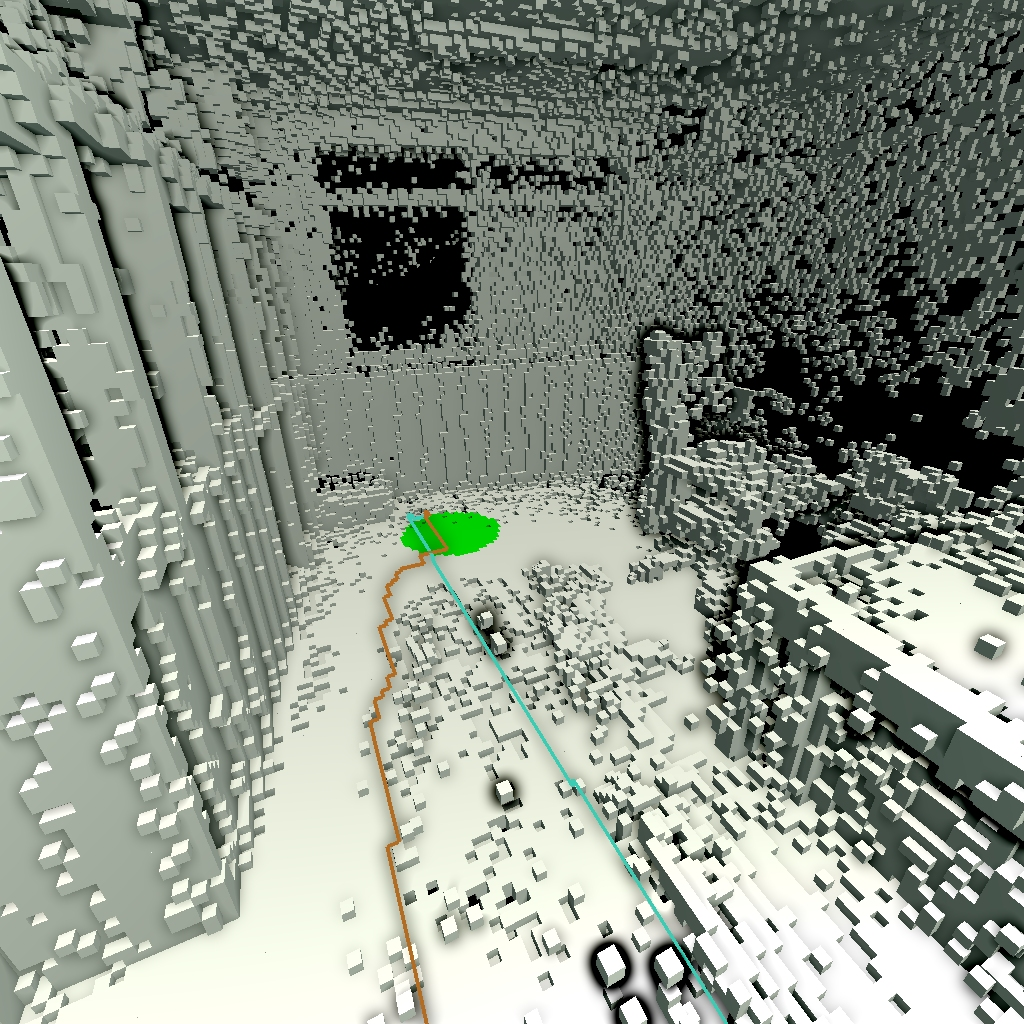
\includegraphics[height=0.25\linewidth]{figures/image1.jpg}}\label{fig:teaser:1}}
	\hfill
	\subfigure[Two of the viable paths in a corridor with two hazardous environments.]{\fbox{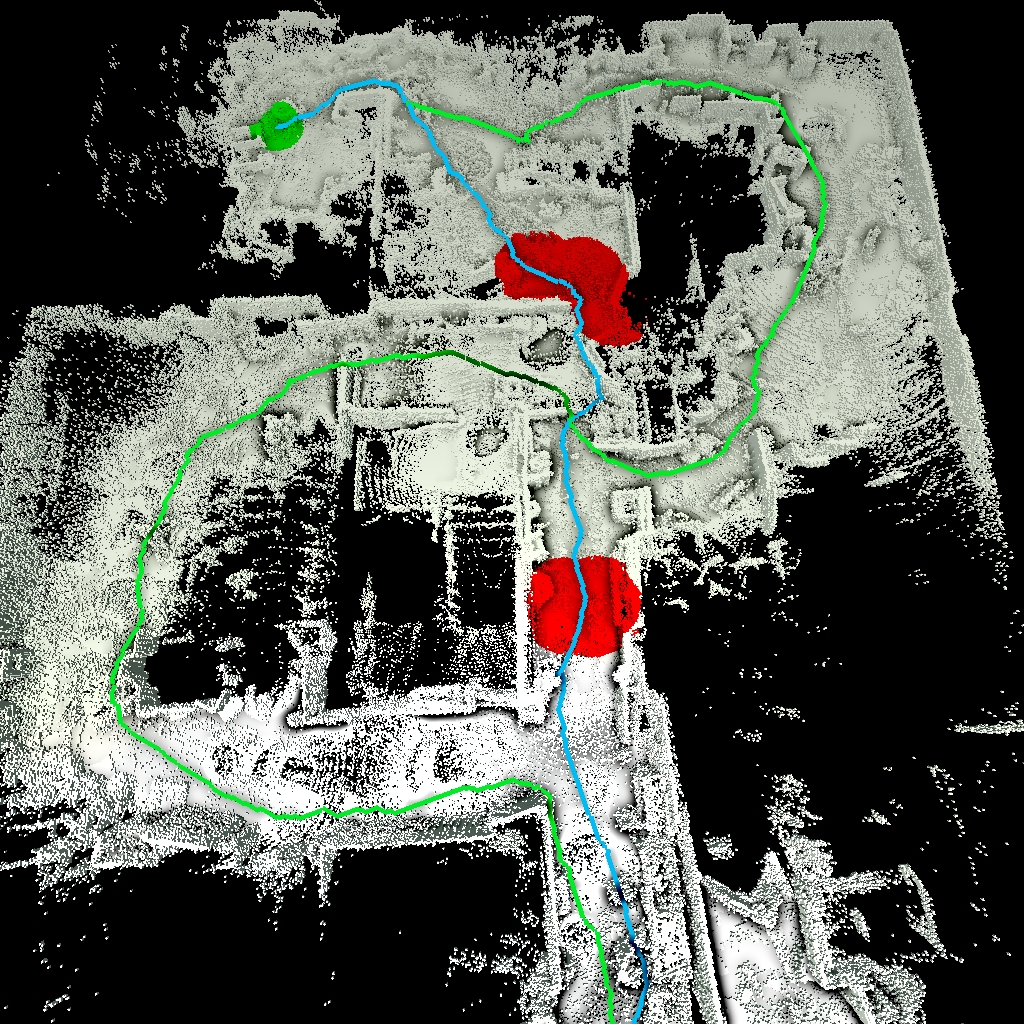
\includegraphics[height=0.25\linewidth]{figures/image2.jpg}}\label{fig:teaser:2}}
	\hfill
	\subfigure[Overhead view of the area in (b) providing context.]{\fbox{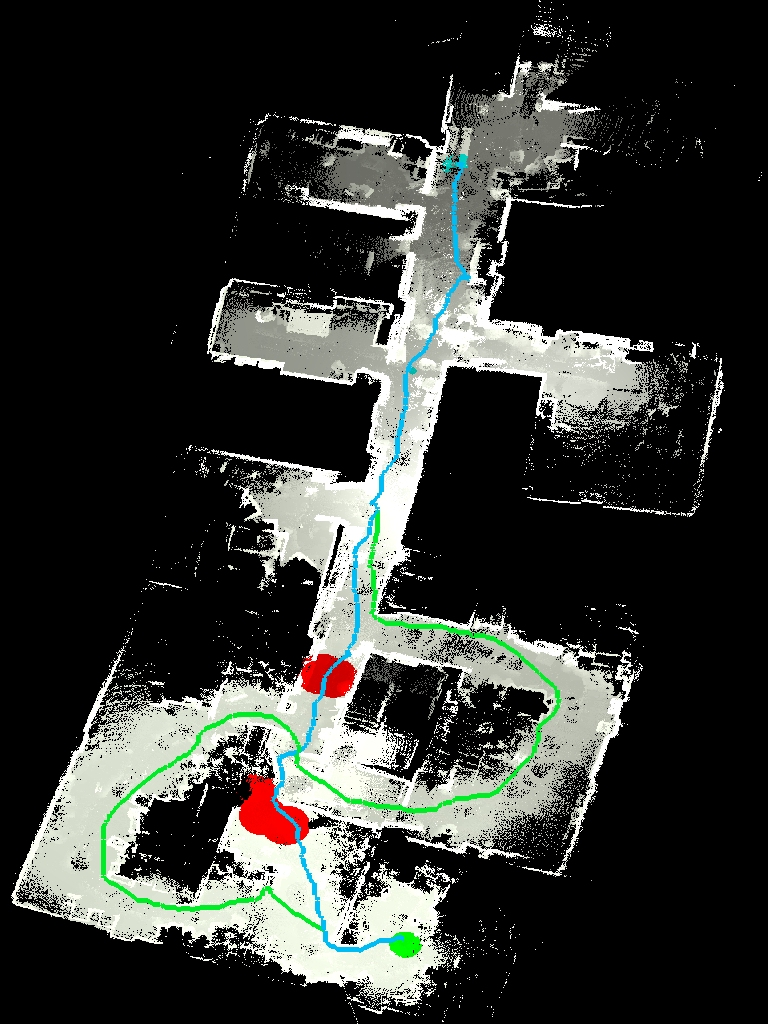
\includegraphics[height=0.25\linewidth]{figures/image2-overview.jpg}}\label{fig:teaser:3}}
	\hfill
	\subfigure[In-depth analysis of an ensemble of paths using parallel coordinates plots and profile plots.]{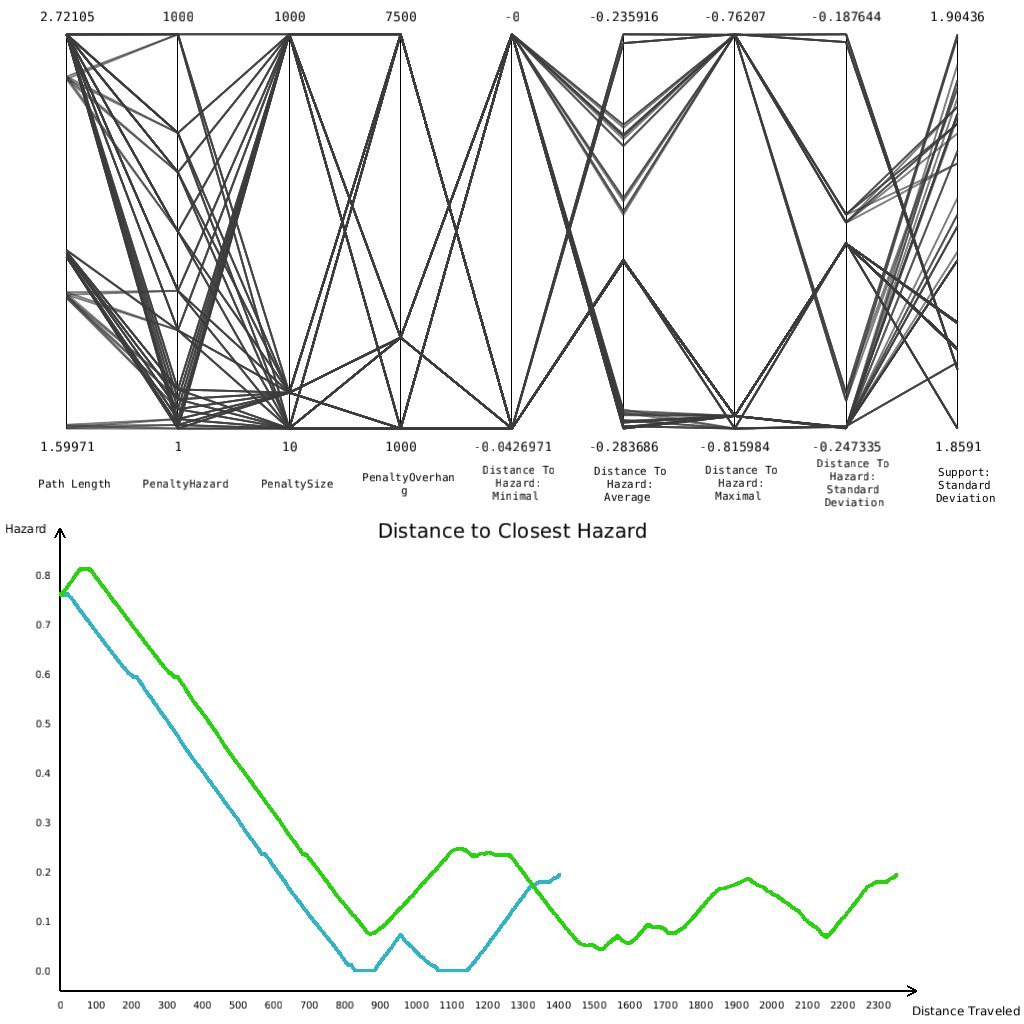
\includegraphics[height=0.25\linewidth]{figures/image4-combined.jpg}\label{fig:teaser:4}}
    \caption{Our visualization system as applied to path planning in the Fukushima Daiichi nuclear reactor site. Different views (a--c) present the operator with a comprehensive understanding of the building, allowing him to select between paths to reach a point-of-interest. The assessment of the trade-off between the paths is supported by a set of visual analysis tools (d).}
    \label{fig:teaser}
}